\documentclass[../main.tex]{subfiles}
\begin{document}
\subsection{关系}
一个集合的元素可与另一个集合的元素形成对应关系。例如,设$A$是所有成年公民的集合,那么“婚姻”就是定义在$A$的任意两个不同元素之间的关系。每对夫妻都是一个有序对$\left(a,b\right)\in A\times A$。在实际社会生活中,我们是先用其他概念对婚姻关系进行定义(例如当地的《婚姻法》),再辨别任意两个公民之间是否具有婚姻关系的。但是在集合论中,我们没有其他超出集合论的其他概念以供我们独立地定义元素间的一种关系。我们只能视符合某关系的\emph{所有}有序对的集合为这一关系的定义。例如,我们不采用既有的《婚姻法》来定义何谓婚姻关系,而是把所有具有婚姻关系的公民对全部列出来组成一个集合,作为关于“何谓婚姻关系”的一种完整的界定。要辩认$a, b\in A$是否婚姻关系,就只看有序对$\left(a,b\right)$是否属于上述集合。这种定义关系的方法才是集合论可以普适地采用的。

正式地,若集合$R$的元素都是有序对,则集合$R$就是一个\emph{关系(relation)}。若有序对$\left(x,y\right)\in R$,则记为$xRy$。习惯上,一般的关系常用符号“$\sim$”表示,各种特殊的关系会用特定的符号表示。设$\sim$是一个关系,若$\left(x,y\right)\in \sim$,则$x\sim y$;若$\left(x,y\right)\notin\sim$,则记为$x\not\sim y$。关系的定义告诉我们:

\begin{figure}[htbp]
    \centering
    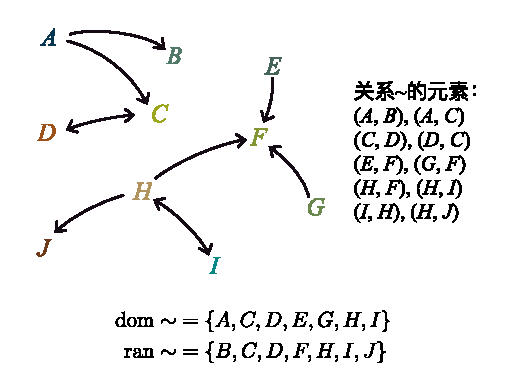
\includegraphics{../images/relation.pdf}
    \caption{图中展示了一个关系$\sim$。箭头表示一个有序对中两个元素的先后次序。}
    \label{fig:II.1.1}
\end{figure}

\begin{enumerate}
    \item 关系$\sim$是一个有序对的集合。图\ref{fig:II.1.1}的箭头表示法可协助我们把“有序对的集合”联系到“关系”一词的日常意义。
    \item 任一关系$\sim$总可以写成两个集合的笛卡尔积的子集。证明的方法:验证关系$\sim$至少可以是下列笛卡尔积
          \[
              \bigcup_{X\in\bigcup_{X^\prime\in\sim}X^\prime}X \times\bigcup_{X\in\bigcup_{X^\prime\in\sim}X^\prime}X
          \]
          的子集\footnote{提示:回顾有序对的定义$\left(a,b\right)\equiv\left\{\left\{a\right\},\left\{a,b\right\}\right\}$,把表达式
              \[
                  \bigcup_{X\in\bigcup_{X^\prime\in\sim}X^\prime}X
              \]
              所形成的集合写出来,可以发现它是关系$\sim$的所有有序对中的元素的集合。读者可以尝试以图\ref{fig:II.1.1}的例子写出图中关系的$\bigcup_{X\in\bigcup_{X^\prime\in\sim}X^\prime}X$;它就是$\left\{A,B,C,D,E,F,G,H,I,J\right\}$。}
    \item 关系的元素未必是同一个集合与其自身的笛卡尔集。两个不同集合$X$与$Y$之间也可以定义某关系$\sim\subset X\times Y$。只要$x\in X,y\in Y,\left(x,y\right)\in\sim$,则$x\sim y$。若$\sim\subset X\times X$,则称“$\sim$是集合$X$上的关系”;若$\sim\subset X\times Y$,则称“$\sim$是从集合$X$到集合$Y$的关系”。
\end{enumerate}

\begin{example}
    设$A=\left\{a,b\right\}, B=\left\{1,2\right\}$,则$A\times B=\left\{\left(a,1\right),\left(a,2\right),\left(b,1\right),\left(b,2\right)\right\}$。设关系$\sim=\left\{\left(a,1\right),\left(b,2\right)\right\}$。我们不难留意到,$\sim\subset A\times B$。按照关系$\sim$的定义,我们可以写$a\sim 1,a\not\sim 2$。

    留意到,$A\times B$本身就是一个关系。若$\sim=A\times B$,则$A$的任一元素与$B$的任一元素之间都有$\sim$关系,即$\forall a\in A\forall b\in B,a\sim b$。

    等于“$=$”关系是任一集合与其自身的笛卡积的子集。具体地,设$X$是一个非空集合,则$X\times X$中所有满足$x=y$的有序对$\left(x,y\right)$的集合就是等于关系。

    属于“$\in$”也是一个关系。具体地,它是$X\times\mathcal{P}\left(X\right)$满足$x\in A$的所有有序对$\left(x,A\right)$的集合。

    空集是有序对的集合(因为空集是集合,且空集不含有任何不是有序对的元素),因此空集也可以是一个关系。
\end{example}

接上列的第2条,给定一个关系$\sim$,记$U_\sim\equiv\bigcup_{X\in\bigcup_{X^\prime\in\sim}X^\prime}X$,遵循分类公理所构建的集合
\[
    \left\{a|a\in U_\sim\wedge\left(\exists b,b\in U_\sim\wedge a\sim b\right)\right\}
\]
为关系$\sim$的\emph{定义域(domain)},记作$\mathrm{dom}\sim$\footnote{式中的记法“$\exists b,\left(\text{关于$b$的语句}\right)$表示“存在符合关于$b$的语句的一个$b$”。例如“$\exists b,b\in U_\sim$”表示“存在一个属于集合$U_\sim$的$b$”。}。集合
\[
    \left\{b|b\in U_\sim\wedge \left(\exists a,a\in U_\sim\wedge a\sim b\right)\right\}
\]
为关系$\sim$的\emph{值域(range)},记作$\mathrm{ran}\sim$。图\ref{fig:II.1.1}给出了所示关系的定义域和值域。不难留意到,对任一关系$\sim$有$\sim\equiv\left(\mathrm{dom}\sim\right)\times\left(\mathrm{ran}\sim\right)$;对于任一集合上的等于关系,有$\left(\mathrm{dom}=\right)=\left(\mathrm{ran}=\right)$;对于任一集合上的属于关系,若$\left(\mathrm{dom}\in\right)=X$,则$\left(\mathrm{ran}\in\right)=\mathcal{P}\left(X\right)\setminus\left\{\emptyset\right\}$\footnote{因为$\emptyset\in\mathcal{P}\left(X\right)$,但没有元素能够属于$\emptyset$。}。

设$\sim$是集合$X$上的一个关系。若
\begin{enumerate}
    \item 对任一$x\in X$都有$x\sim x$,则称关系$\sim$是\emph{自反的(reflextive)}。如果图\ref{fig:II.1.1}中的每个元素都有一个从自己回到自己的箭头,那么图中的关系就是自反的。
    \item 对任意$x\in X$和$y\in X$,只要$x\sim y$就有$y\sim x$,则称关系$\sim$是\emph{对称的(symmetric)}。如果图\ref{fig:II.1.1}中的所有箭头都是双向箭头,那么图中的关系就是对称的。
    \item 对任意$x\in X$、$y\in X$和$z\in X$,只要$x\sim y\text{且}y\sim z$就有$x\sim z$,则称关系$\sim$是\emph{传递的(transitive)}。读者可尝试把图\ref{fig:II.1.1}的关系修改成非自反、非对称,但传递的关系\footnote{注意这几条定义所要求的“对任意……”,只要有一个例外就可以失效。}。
\end{enumerate}
若集合$X$上的一个关系$\sim$同时满足上述3个性质,则称$\sim$是$X$上的一个\emph{等价关系(equivalent relation)}。

\begin{example}
    设$X=\left\{a,b,c\right\}$。请验证,$X$上的等于关系是集合
    \[
        \left\{\left(a,a\right),\left(b,b\right),\left(c,c\right)\right\}
    \]
    共有3个元素;$X\times X$也是$X$上的等价关系,它有$2^3=8$个元素。

    一般地,任一非空集合$X$上的等于关系是$X$上的(除空集外)“最小”的等价关系,$X\times X$是$X$上的最大等价关系。

    显然,“婚姻”不是“全体成年公民”集合上的等价关系。“婚姻”只满足对称性。
\end{example}

如果集合$X$的非空子集的集合$\mathcal{C}$满足$\bigcup_{Y\in\mathcal{C}}Y=X$且$\mathcal{C}$的元素两两不相交,则称集合$\mathcal{C}$是$X$的一个\emph{划分(partition)}。换言之,如果$X$的若干个非空子集两两不相交,但它们的并集又恰好得到$X$,那么这些子集就好像对集合$X$进行“切蛋糕”所得到结果(如图\ref{fig:II.1.2}所示)。不难留意到$\mathcal{C}\subset\mathcal{P}\left(X\right)$。

\begin{figure}[htbp]
    \centering
    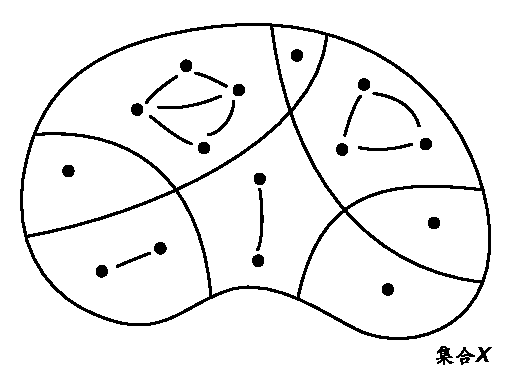
\includegraphics[width=0.5\textwidth]{../images/partition.pdf}
    \caption{集合的划分示意图}
    \label{fig:II.1.2}
\end{figure}

设关系$\sim$是集合$X$上的一个等价关系,则集合$\left\llbracket x\right\rrbracket_\sim\equiv\left\{y|y\in X\text{且}\exists x\in X,y\sim x\right\}$称$x$关于$\sim$的\emph{等价类(equivalent class)}\footnote{“类”与“集合”在概念上无实质区别。}。$X$的元素关于$\sim$的所有等价类的集合,记作$X/\sim$\footnote{注意与相对补集的符号相区别。},称为集合$X$在等价关系$\sim$下的\emph{商集(quotient set)}\footnote{正式地,
    \[
        X/\sim\equiv\left\{A|A\in\mathcal{P}\left(X\right)\wedge\left(\forall x\in A,\left\llbracket x\right\rrbracket_\sim = A\right)\right\}
    \]
}。仍以图\ref{fig:II.1.2}为例。圆点表示集合$X$的元素。在集合$X$上定义了等价关系,圆点之间的连线是双向的。每个元素,都能通过这一等价关系的传递性联系若干个共同关联的元素,而形成$X$的一个子集。每个这样的子集,都是$X$关于这一等价关系的等价类。

若集合$\mathcal{C}$是集合$X$的一个划分,我们可以定义一个关系$\sim\equiv X/\mathcal{C}$\footnote{该记法与刚刚介绍完的$X/\sim$无关,是符号“$/$”的滥用。},使得当且仅当$X$的元素$x,y$属于$\mathcal{C}$的同一个元素时,$x\sim y$。此时我们称关系$\sim$是\emph{由集合$X$的划分$\mathcal{C}$引出的关系(equivalent relation induced by the partition $\mathcal{C}$ of $X$)}。\footnote{正式地,
    \[
        X/\mathcal{C}=\left\{\left(x,y\right)|\left(x,y\right)\in X\times X\wedge\left(\exists A\in \mathcal{C},\left\{x,y\right\}\subset A\right)\right\}
    \]
}
可以证明,\emph{集合$X$上的任一划分都唯一地引出一个$X$上的等价关系}\footnote{\href{https://proofwiki.org/wiki/Relation_Induced_by_Partition_is_Equivalence}{证明过程}}。仍以图\ref{fig:II.1.2}为例,我们可以让集合$X$上的这一划分下每个子集内的元素之间都建立关系。这种关系可描述为“$X$的两个元素同属$X$的划分的同一个元素”\footnote{理解此句时注意$X$的划分是$X$的子集的集合,其元素是$X$的子集。图\ref{fig:II.1.2}中的连续,不过是把同属于一个子集的所有元素两两相连。}。易验这种关系是等价关系。因此$X$的任一划分,都能用这种描述使得每一划分都是$X$关于某等价关系的等价类。故我们总是可以直接说$X/\mathcal{C}$是由集合$X$的划分$\mathcal{C}$引出的等价关系。这一关系的“唯一性”,意思是说,不会有另一个$X$上的不同的等价关系\footnote{等价关系是集合。故等价关系“相同”即集合的相等;“不同”既集合的不相等。集合的相等已经在上一节定义过。}。

\begin{theorem}[等价关系基本定理]
    设$\sim\subset X\times X$是集合$X$上的一个等价关系,则$X$在$\sim$下的商集$S/\sim$是$S$的一个划分。
\end{theorem}
\begin{proof}
    根据划分的定义,要使$S/\sim$是$S$的一个划分,以下3条必须同时满足:
    \begin{enumerate}
        \item $S/\sim$的元素都不是空集,即$\forall\left\llbracket x\right\rrbracket_\sim\in S/\sim,\left\llbracket x\right\rrbracket_\sim\neq\emptyset$;
        \item $S/\sim$的元素两两不交,即$\left\llbracket x\right\rrbracket_\sim\neq\left\llbracket y\right\rrbracket_\sim\Leftrightarrow\left\llbracket x\right\rrbracket_\sim\cap\left\llbracket y\right\rrbracket_\sim=\emptyset$;
        \item 所有$S/\sim$的元素并集得到集合$S$,即$\bigcup_{Y\in S/\sim}Y=S$。
    \end{enumerate}
    具体证明过程暂略\footnote{\href{https://proofwiki.org/wiki/Fundamental_Theorem_on_Equivalence_Relations}{证明过程}}。
\end{proof}

由等价关系基本定理,我们可以写
\[
    \sim=X/\mathcal{C}\Leftrightarrow \mathcal{C}=X/\sim
\]
这使得等价关系、划分和商集有类似“集合的除法”的意义。该定理告诉我们,集合上的一个等价关系必定可以划分这个集合。
\end{document}